\section{صفحه نمایش \lr{LCD} و صفحه کلید ماتریسی}

\subsection{اهداف آزمایش}
\begin{itemize}
    \item آشنایی با صفحه نمایش \lr{LCD} و صفحه کلید ماتریسی به عنوان رابط های کاربری
    \item آشنایی با نحوه‌ی اضافه کردن کتاب‌خانه ها در محیط آردوینو
\end{itemize}

\subsection{قطعات مورد نیاز}
\begin{itemize}
    \item \lr{Arduino Uno}
    \item صفحه نمایش \lr{LCD}
    \item صفحه کلید ماتریسی
    \item پتانسیومتر ۱ کیلواهم \lr{B1K}
    \item مقاومت ۲۲۰ اهم
\end{itemize}
\pagebreak

\subsection{مقدمه}

\begin{nas}یاد آوری مقسم ولتاژ و پتانسیومتر\end{nas}
\newline
در درس و آزمایشگاه مدار های الکتریکی با مدار مقسم ولتاژ آشنا شدید. این مدار در واقع از ۲ مقاومت سری تشکیل شده که ولتاژ ورودی میان آنها تقسیم می‌شود.
\newline
\begin{figure}[h]
    \centering
    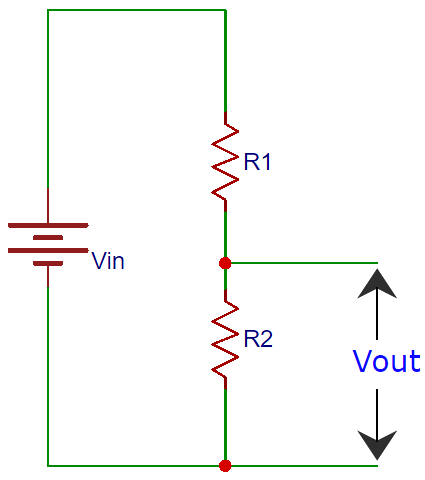
\includegraphics[width=4cm]{vdiv.png}
    \caption{مدار مقسم ولتاژ}
    \label{fig:voldiv}
\end{figure}
\newline
با استفاده از \lr{KVL} به سادگی به فرمول زیر می‌رسیم:
\begin{equation}V_{out} = V_{in} \times \frac{R2}{R1 + R2}\end{equation}
استفاده‌ی اصلی ما از این مدار، کم کردن ولتاژ ورودی به یک وسیله‌است. پتانسیومتر ها مقسم های ولتاژی هستند که مقدار مقاومت های \lr{R1} و \lr{R2}در آنها (معمولا با چرخاندن سر پتانسیومتر) قابل تغییر است و در این آزمایش برای کنترل کنتراست صفحه نمایش از آن استفاده می‌کنیم.
\newline
\begin{figure}[h]
    \centering
    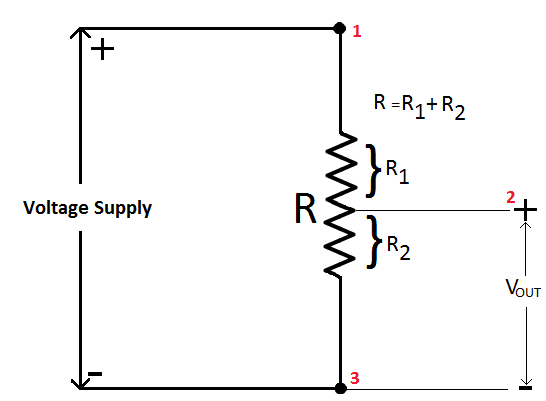
\includegraphics[width=8cm]{pot.png}
    \caption{مدار معادل یک پتانسیومتر. توجه کنید هنگامی که می‌گوئیم یک پتانسیومتر ۱۰ کیلو اهمی، ۱۰ کیلو اهم بیانگر مقدار \lr{R} است.}
    \label{fig:pot-circ}
\end{figure}
\newline
\begin{nas}صفحه نمایش \lr{LCD}\end{nas}
\newline
صفحه نمایش کاراکتری \lr{16x2} یکی از روش های متداول ارتباط با کاربر در سیستم های نهفته‌است. منظور از \lr{16x2} اندازه‌ی صفحه نمایش است، یعنی این صفحه های نمایش قابلیت نشان دادن ۲ ردیف و ۱۶ ستون از کاراکتر ها را دارند. خود صفحه نمایش توسط یک \lr{IC} کنترل می‌شود که میکروکنترلر ما باید با آن ارتباط برقرار کند. ابتدا با پین های ورودی یک ماژول صفحه‌نمایش کاراکتری آشنا می‌شویم:
\newline
\begin{figure}[h]
    \centering
    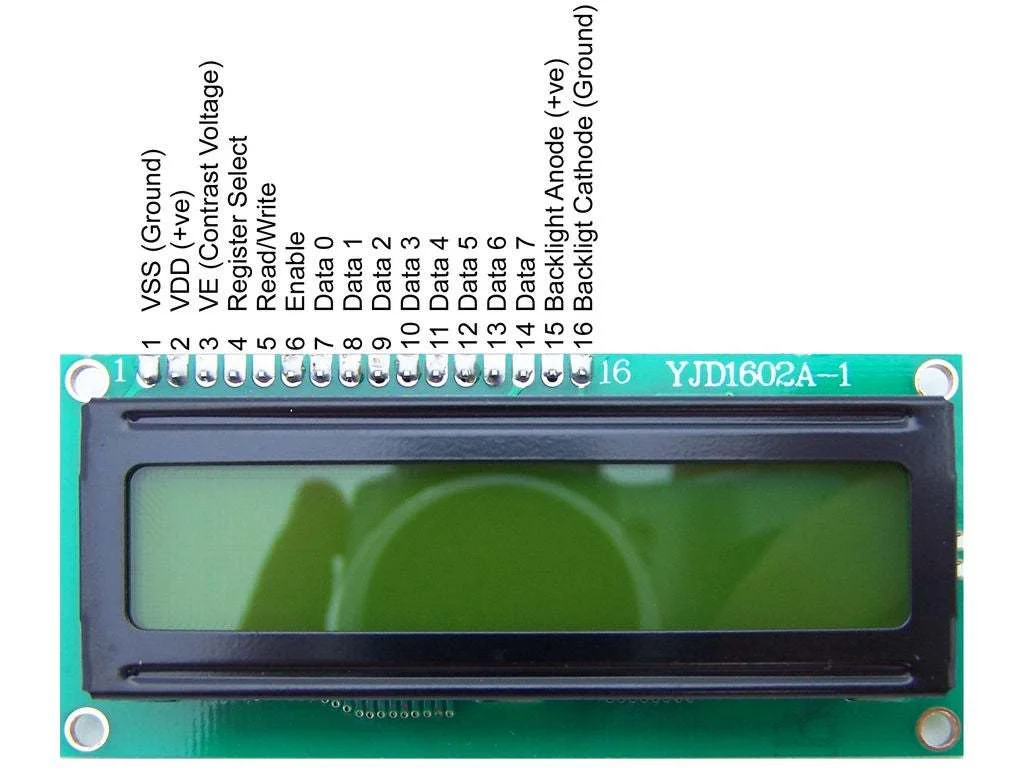
\includegraphics[width=8cm]{lcd_pinout.png}
    \caption{نمایی از یک صفحه نمایش کاراکتری ۱۶ در ۲}
    \label{fig:lcd-pinout}
\end{figure}
\begin{itemize}
    \item پین شماره ۱: ولتاژ \lr{Ground}
    \item پین شماره ۲: ولتاز \lr{Vcc}
    \item پین شماره ۳: کنترل کنتراست. با استفاده از یک پتانسیومتر می‌توانیم کنتراست صفحه نمایش را کنترل کنیم
    \item پین های شماره ۴ تا ۶: پین های کنترلی
    \item پین های شماره ۷ تا ۱۴:‌پین های ورودی داده
    \item پین های شماره ۱۵ و ۱۶: به ترتیب آنود و کاتود \lr{Backlight LED}. توجه کنید این پین ها مستقیما به یک \lr{LED} متصل می‌شوند و ارتباطی با آی‌سی کنترلر ندارند. طبیعتا مانند دیگر \lr{LED} ها حتما برای جلوگیری از خرابی قطعه باید یک مقاومت با آن سری قرار دهید.
\end{itemize}
\pagebreak
از آنجایی که ما از کتاب‌خانه های مخصوص ارتباط با \lr{LCD} استفاده خواهیم کرد، نیازی به دانستن جزئیات این ارتباط نیست و در صورت علاقه می‌توانید خودتان از دیتاشیت مربوطه مطالعه کنید، اما باید نحوه‌ی کار با کتابخانه را بلد باشید و بتوانید از آن استفاده کنید.
\newline
\textcolor{red}{\begin{nas}سوال: \end{nas}}
\newline
در مورد توابع زیر از کتابخانه‌ی \lr{LiquidCrystal.h} تحقیق کنید و ورودی و خروجی توابع و کاری که انجام می‌دهند را بنویسید.
\begin{itemize}
    \item \lr{LiquidCrystal()}
    \item \lr{begin()}
    \item \lr{clear()}
    \item \lr{home()}
    \item \lr{setCursor()}
    \item \lr{write()}
    \item \lr{print()}
\end{itemize}

\pagebreak
\begin{nas}صفحه کلید ماتریسی\end{nas}
\newline
در آزمایش قبلی از کلید های معمولی برای گرفتن ورودی از کاربر استفاده کردیم. اگر بخواهیم مانند روش آزمایش قبل ۱۶ عدد کلید برای ورودی داشته باشیم به مشکل می‌خوریم، چون تعداد پین های ورودی میکروکنترلر ما محدود است. به همین دلیل باید از روش ماتریسی برای اتصال کلید ها به میکروکنترلر استفاده کنیم.
\newline
در این روش کلید ها به صورت زیر در یک جدول قرار می‌گیرند:
\newline
\begin{figure}[h]
    \centering
    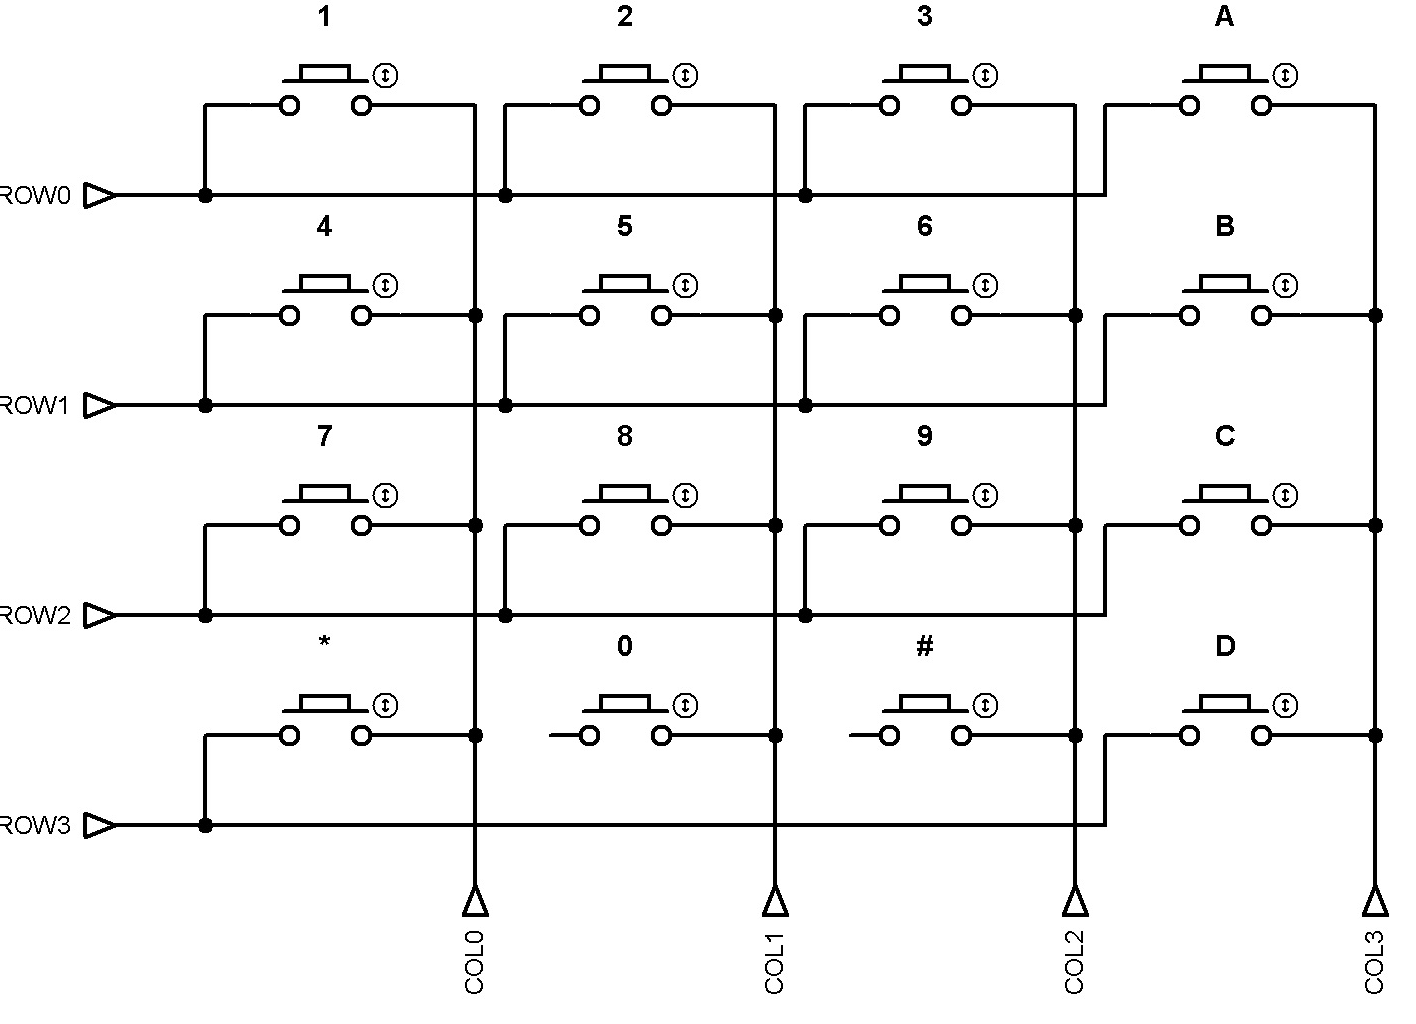
\includegraphics[width=16cm]{keypad-circ.png}
    \caption{مدار یک صفحه کلید ماتریسی}
    \label{fig:keypad-circ}
\end{figure}
\newline
برای استفاده از این مدار، باید به همه‌ی سطر ها ولتاژ صفر منطقی بدهیم و ستون ها را با استفاده از
\lr{Pull Up Resistor} به ورودی های میکروکنترلر وصل کنیم.
هنگامی که یک کلید بسته می‌شود سطر و ستون متناظر با آن متصل می‌شوند و ورودی آن ستون به میکروکنترلر از یک به صفر منطقی تغییر پیدا می‌کند. در این مرحله می‌دانیم که یک کلید در ستونی که ورودیش تغییر کرده روشن شده است. برای اینکه سطر آن را نیز پیدا کنیم و بفهمیم کدام کلید روشن شده، یک به یک سطر ها را به یک منطقی تغییر می‌دهیم. اگر هنگامی که یک سطر به یک منطقی تغییر کرد، ستون نیز به یک منطقی تغییر کند سطری که کلید در آن قرار دارد را نیز پیدا کرده‌ایم و تشخیص دادیم که کدام کلید بسته شده بود.

\newline
\textcolor{red}{\begin{nas}سوال: \end{nas}}
شبه کد/فلوچارت استفاده از صفحه کلید ماتریسی را بنویسید.
\newline

برای کار با صفحه کلید نیز از کتاب‌خانه های مخصوص به آن استفاده می‌کنیم که نام آن \lr{Keypad.h} است.
برای دریافت این کتاب‌خانه، از منوی سمت راست \lr{Arduino IDE} به قسمت \lr{Library Manager} بروید و کتابخانه‌ی \lr{Keypad by Mark Stanley} را دریافت نمایید. مستندات مربوط به این کتاب‌خانه را می‌توانید در 
\href{https://playground.arduino.cc/Code/Keypad/}{این لینک}
مشاهده کنید.
\newline
\textcolor{red}{\begin{nas}سوال: \end{nas}}
در مورد توابع زیر از کتابخانه‌ی \lr{Keypad.h} تحقیق کنید و ورودی و خروجی توابع و کاری که انجام می‌دهند را بنویسید.
\begin{itemize}
    \item \lr{Keypad()}
    \item \lr{begin()}
    \item \lr{waitForKey()}
    \item \lr{getKey()}
\end{itemize}
\newline
\subsection{شرح آزمایش}

می‌خواهیم یک ماشین‌حساب درست کنیم. ابتدا مانند مداری که در انتهای آزمایش در اختیار شما قرار گرفته، صفحه نمایش و صفحه کلید را به آردوینو متصل کنید. نیازی نیست مدار شما دقیقا همان مدار باشد، اما توجه کنید که به هیچ عنوان قرار دادن مقاومت و پتانسیومتر در مدار را فراموش نکنید. در صورتی که پتانسیومتر ندارید، می‌توانید به پین \lr{Vo} یک مقاومت ۳.۳ کیلواهمی متصل به زمین وصل کنید. همچنین وقتی صفحه کلید ماتریسی رو به روی شما باشد و پین‌ها رو به پایین باشند، پین‌ها از چپ به راست ابتدا پین های ردیف‌ها هستند و سپس پین های ستون‌ها هستند. برنامه‌ای بنویسید که کلید ها را از صفحه کلید بخواند و آنها را روی صفحه‌نمایش نمایش دهد و بعد از اینکه کلید \lr{=} زده شد، عبارت ریاضی که کاربر وارد کرده را محاسبه کرده و مقدار آن را روی صفحه‌نمایش نمایش دهد.
توجه کنید نیازی به رعایت اولویت ها و پشتیبانی از اعداد اعشاری و اعداد منفی نیست.

\begin{figure}[h]
    \centering
    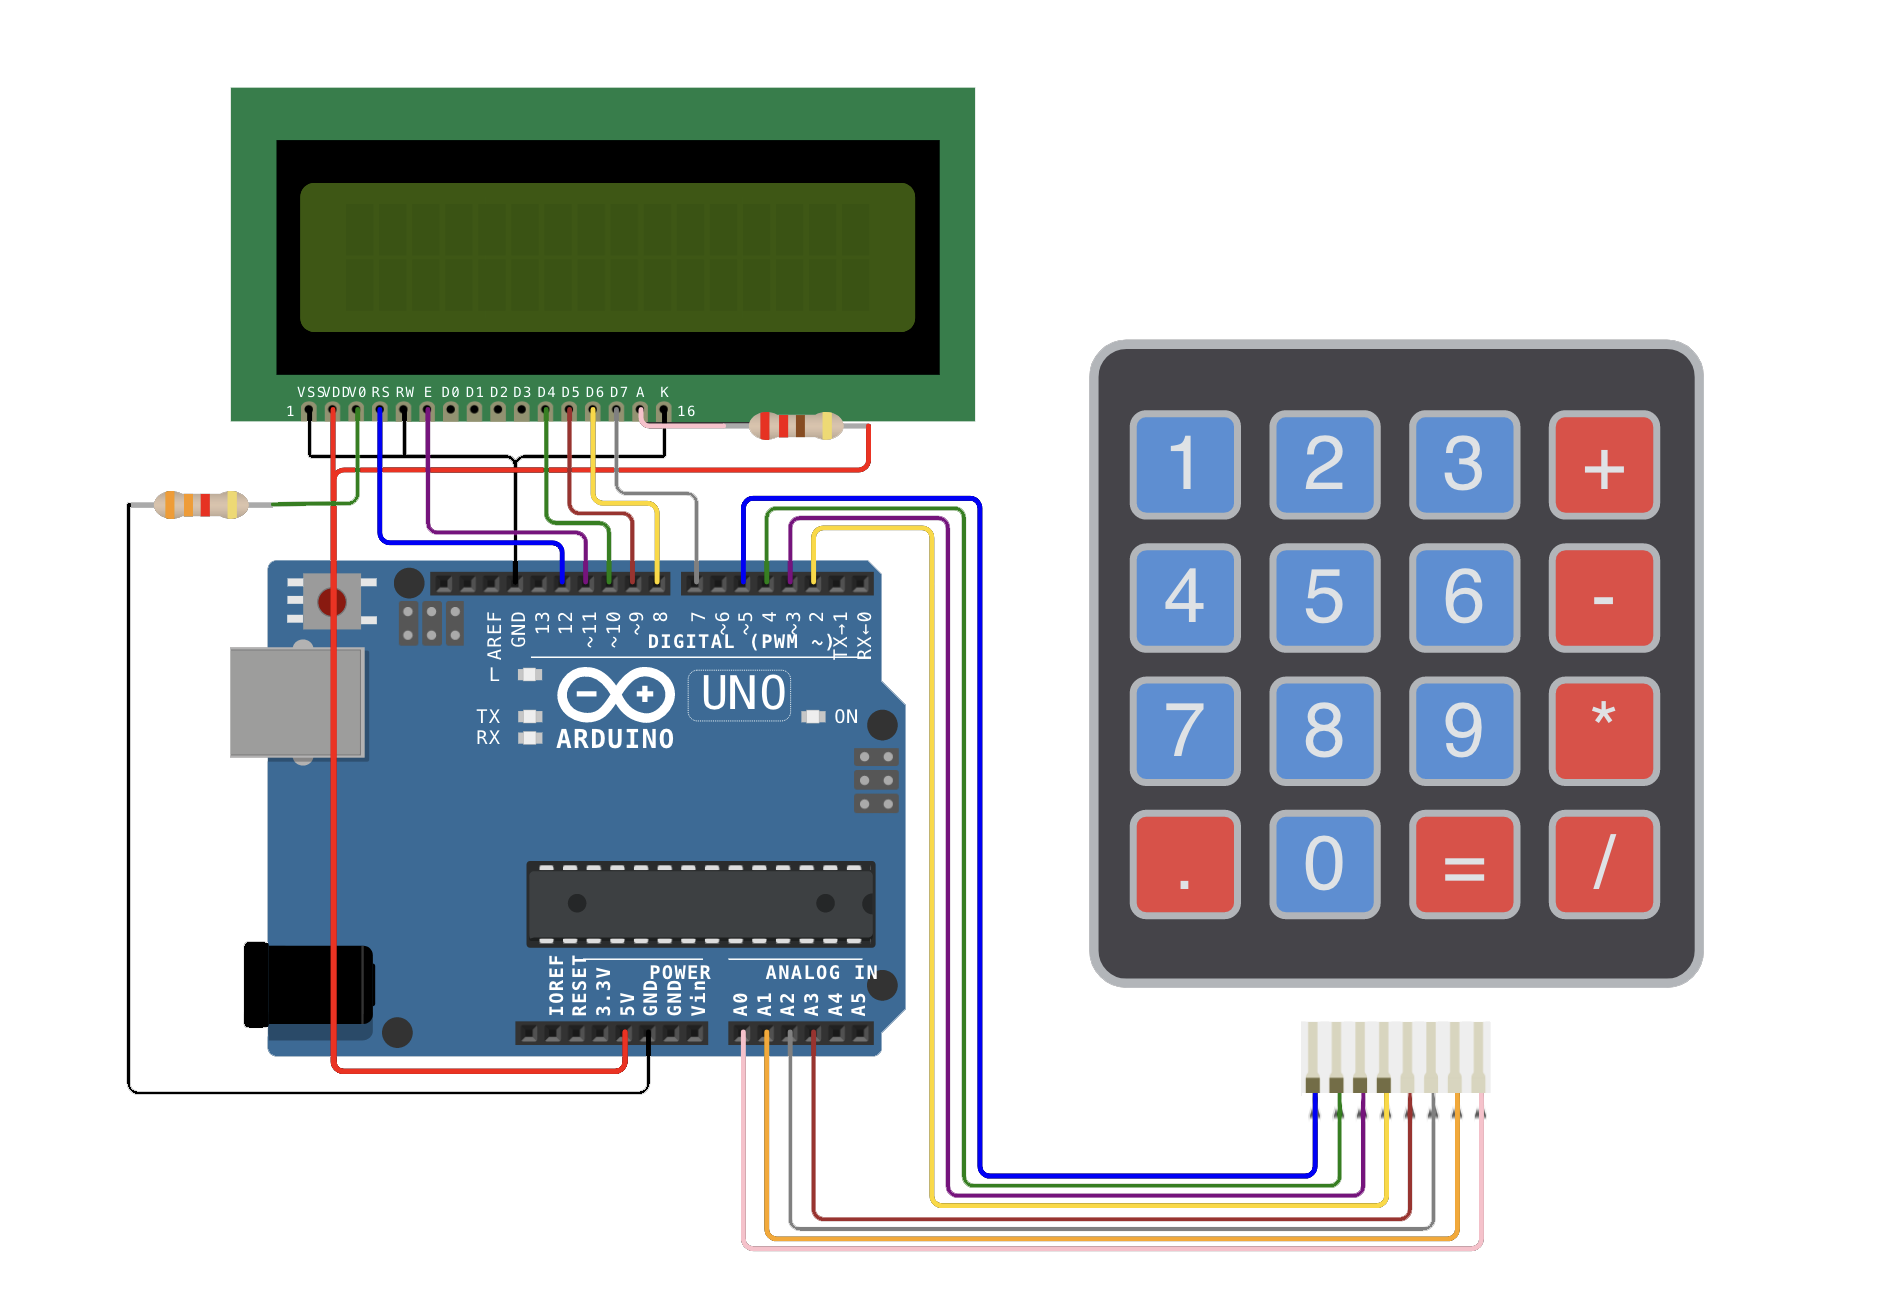
\includegraphics[width=14cm]{L2-Circuit.png}
    \caption{مدار مربوط به آزمایش دوم}
    \label{fig:l2-circ}
\end{figure}

\newline